% LEXICAL STRESS ERRORS
%
% !TEX root = ../thesis-main.tex
%

\chapter{Lexical stress errors by French learners of German}

%\cleanchapterquote{You can’t do better design with a computer, but you can speed up your work enormously.}{Wim Crouwel}{(Graphic designer and typographer)}

%\blindtext

\section{Stress in German vs. French }
	\subsection{Comparative prosody}
	\subsection{Stress ``deafness'' in French}
	\subsection{Expected errors}
	
	
	
\section{Lexical stress errors in the IFCASL corpus} 

	To investigate to what extent the expected lexical stress errors by French speakers of German are actually produced, a subset of the non-native German-language IFCASL corpus was annotated for such errors, with a view to answering the following questions:

	\begin{itemize}
	\item{Are lexical stress errors observed frequently in the IFCASL data?}
	\item{Is there a difference in the frequency of these errors among different groups of speakers (i.e. in terms of skill level, age, or gender) or in different contexts (e.g. after hearing a native speaker produce the word)?}
	\item{Are lexical stress errors observed more frequently with certain word types than with others?}
	\item{Can lexical stress errors be reliably identified by native German speakers (i.e. to what extent do the judgments of different annotators agree)?}
	\item{Are there differences in how native and non-native German speakers annotate stress errors?}
	\item{How frequently do technical problems interfere with determining the accuracy of a production?}
	\end{itemize}
	
	
	\subsection{Data}
	
	The IFCASL sub-corpus annotated for lexical stress errors consists of utterances of twelve word types (see \cref{tab:bisyllwords}), each of which is bisyllabic and canonically has its primary stress on the initial syllable. These characteristics were chosen deliberately: the selected words are bisyllabic because this simplifies comparison between stressed and unstressed syllables, and they are initial-stress because this is the stress pattern which L1 French speakers are expected to have the most difficulty producing in German, given the fixed final-position stress and final lengthening in French.
	
	In the IFCASL corpus recordings, sentences containing these words were read aloud by L1 and L2 (L1 French) speakers. Here, only the L2 utterances were annotated; it is assumed that the L1 German speakers always realize lexical stress correctly. 
	%The recordings were performed under two conditions: the ``Sentence Read'' (SR) condition, in which the L2 speaker is simply  presented with the text of the sentence and asked to record themselves reading it aloud, and the ``Sentence Heard'' (SH) condition, in which the L2 speaker is asked to listen to an utterance of the sentence by an L1 German speaker before recording their own utterance.
	Utterances (tokens) of each word as produced by over 50 L2 speakers were extracted from the recordings automatically in Praat \parencite{Boersma2014}, using the word-level segmentation of each sentence utterance automatically obtained by forced alignment (see \TODO{ref}).
	
	\begin{table}[htb]
		\centering
		\caption{The twelve bisyllabic initial-stress words types selected from the IFCASL corpus for stress error annotation \TODO{column details}%, and the number of distinct tokens annotated (each produced by a different speaker)
		}
%		\begin{tabular}{llll}
%		Flagge & Ringen & Tschechen & halten \\
%		M\"{o}rder & Tatort & Fr\"{u}hling & fliegen \\
%		Pollen & manche & E-mail & tragen \\
%		\end{tabular}
		
		\begin{tabularx}{\textwidth}{lXXXXX}
		\toprule
		
		Orthography & 
		Canonical \linebreak pronunciation & 
		Part of speech & 
		English \linebreak translation & 
		Recording condition & 
		Tokens \linebreak annotated\\
		
		\midrule
		E-mail	&	\TODO{prons} &	noun &	e-mail &	SR 	&	56	\\
		Flagge	&	&	noun &	 flag &	SH	&	55	\\
		fliegen	&	&	verb &	fly &	SR		& 56	\\
		Frühling	&	& noun	&	spring &	SR		&	56	\\
		halten	&	&	verb &	hold &	SR 	&	56	\\
		manche	&	&	pronoun &	some & 	SR 	&	56	\\
		Mörder	&	&	noun &	murderer &	SR 	&	56	\\
		Pollen	&	&	noun &	pollen &	SR 	& 	55	\\
		Ringen	&	&	noun &	rings &	SH	&	55	\\
		Tatort	&	&	noun &	crime scene & 	SR 	&		56	\\
		tragen	&	&	verb &	wear &	SH	&	55	\\
		Tschechen	&	& noun	&	Czechs	&	SR		& 56	\\
		\bottomrule
		\end{tabularx}
		\label{tab:bisyllwords}
	\end{table}

	\subsection{Annotation method}

	

	
	The interface of the graphical annotation tool, scripted in Praat \parencite{Boersma2014}, is shown in \cref{fig:annotationtool}. At the top, a word's text is displayed, along with the ID number of the speaker whose utterance of that word will be annotated. The recording of the word, extracted from a longer sentence, is played automatically. The annotator may choose to play the word again, or play the entire sentence; either may be played as many times as the annotator wishes. Once the annotator has judged the accuracy of the lexical stress realization in this utterance, they log that judgment by clicking on one of the gray buttons. The annotator is then automatically advanced to the next utterance, with the counts in the lower right corner tracking their progress towards the total number of tokens to be annotated. 
	
		\begin{figure}[bht]
			\centering
			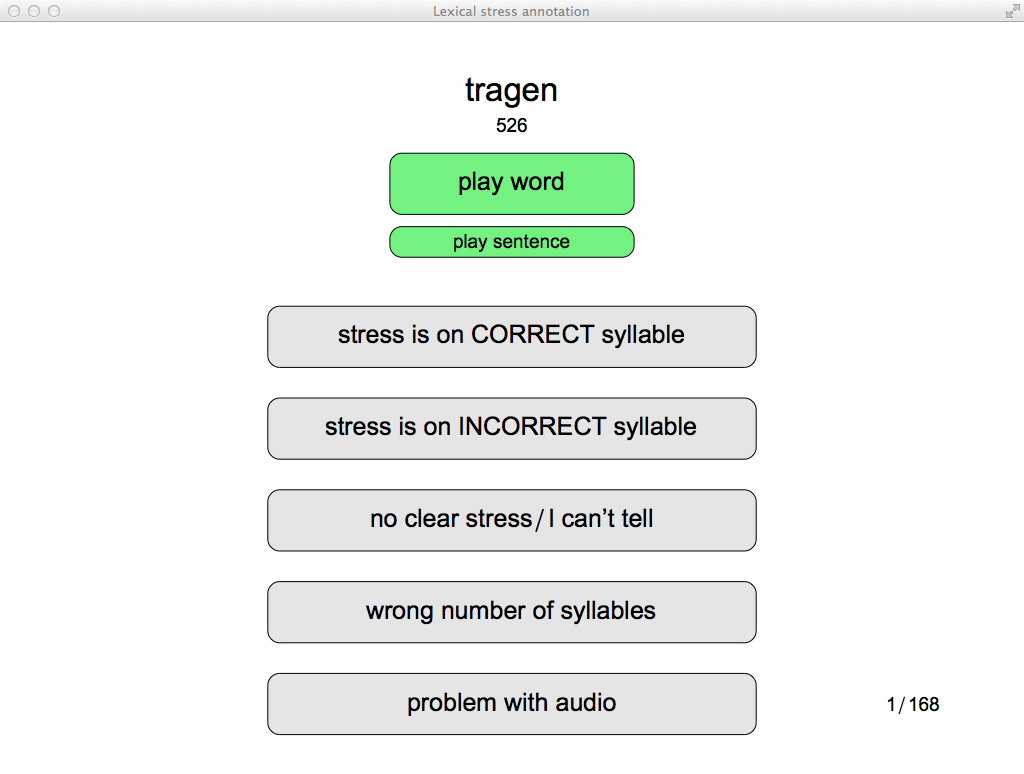
\includegraphics[width=\textwidth]{../img/screenshots/AnnotationTool}
			\caption{A screenshot of the graphical annotation tool scripted in Praat.  }
			\label{fig:annotationtool}
		\end{figure}
	
	\subsection{Results}
	
	\TODO{put some intro text here}
	
	
		\subsubsection{Native vs. nonnative annotators}

		Of the \TODO annotators, \TODO were native German speakers, \TODO{2} were native speakers of American English, and \TODO{one} annotator's first language was Hebrew. 

		In comparing the relative frequencies of the different response classes, we observe that the native and nonnative speakers judge utterances as having correct lexical stress with approximately the same frequency. However, nonnative speakers seem to choose the ``no clear stress/I can't tell'' somewhat more frequently than native speakers; this could be attributed to nonnative speakers being less confident about the how stress should be realized in German, resulting in less certainty about whether a given utterance is correct or not. \TODO{update/verify this paragraph}
		
		\subsubsection{Accuracy by L2 skill level}
		
		
		
		\subsubsection{Accuracy by word type}

%\section{Frequency of production}
%\section{Impact on Intelligibility}
%\section{Automatic detection}